\documentclass[tikz,border=8pt]{standalone}
\usepackage[T1]{fontenc}
\usepackage{lmodern}
\renewcommand{\familydefault}{\sfdefault}
\usetikzlibrary{arrows.meta,positioning,fit}
\definecolor{navy}{HTML}{123C68}
\definecolor{teal}{HTML}{087F86}
\definecolor{amber}{HTML}{C88908}
\begin{document}
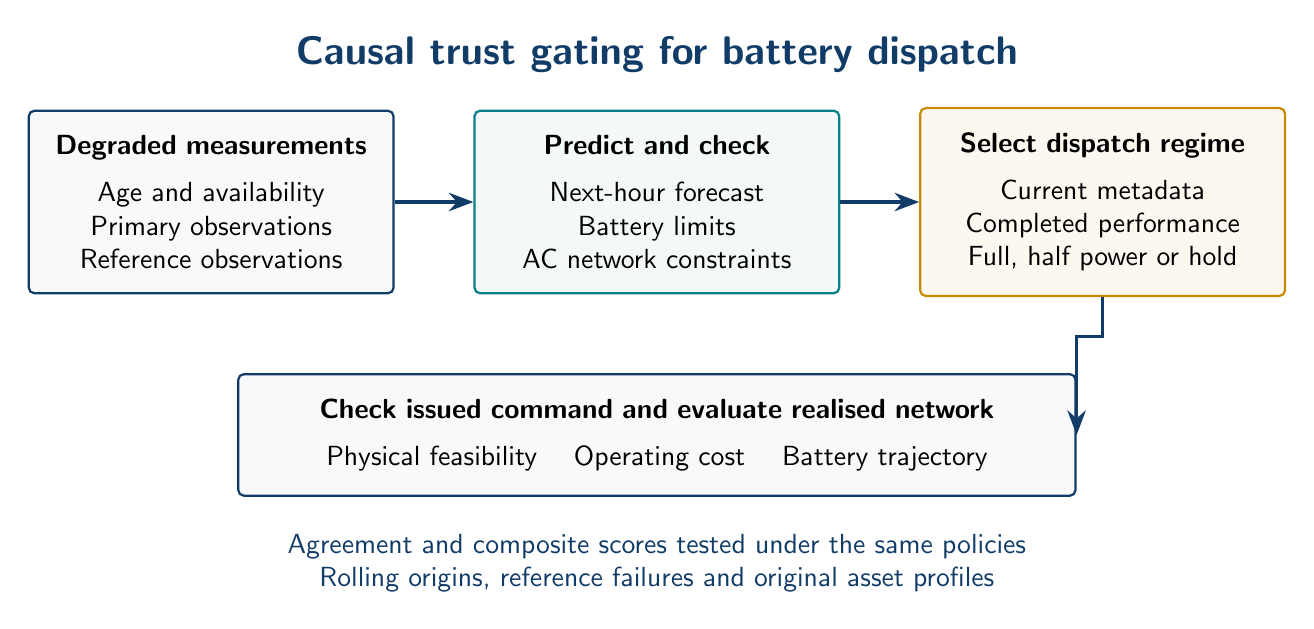
\begin{tikzpicture}[font=\sffamily,>=Stealth,
box/.style={draw=navy,rounded corners=2pt,line width=.8pt,fill=navy!3,
text width=4cm,minimum height=2cm,align=center,inner sep=9pt},
arr/.style={->,draw=navy,line width=1.3pt}]
\node[box] (meter) {\textbf{Degraded measurements}\\[5pt]
Age and availability\\Primary observations\\Reference observations};
\node[box,right=1cm of meter,draw=teal,fill=teal!5] (proposal) {\textbf{Predict and check}\\[5pt]
Next-hour forecast\\Battery limits\\AC network constraints};
\node[box,right=1cm of proposal,draw=amber,fill=amber!6] (gate) {\textbf{Select dispatch regime}\\[5pt]
Current metadata\\Completed performance\\Full, half power or hold};
\draw[arr] (meter)--(proposal);
\draw[arr] (proposal)--(gate);
\node[box,below=1cm of proposal,text width=10cm,minimum height=1.35cm] (plant) {\textbf{Check issued command and evaluate realised network}\\[5pt]
Physical feasibility \quad Operating cost \quad Battery trajectory};
\draw[arr] (gate.south)--++(0,-.5)-|(plant.east);
\node[above=.35cm of proposal,font=\sffamily\bfseries\Large,text=navy] {Causal trust gating for battery dispatch};
\node[below=.35cm of plant,align=center,text=navy] {Agreement and composite scores tested under the same policies\\
Rolling origins, reference failures and original asset profiles};
\end{tikzpicture}
\end{document}
